%%%%%%%%%%%%%%%%%%%%%%%%%%%%%%%%%%%%%%%%%
% The Legrand Orange Book
% LaTeX Template
% Version 2.1.1 (14/2/16)
%
% This template has been downloaded from:
% http://www.LaTeXTemplates.com
%
% Original author:
% Mathias Legrand (legrand.mathias@gmail.com) with modifications by:
% Vel (vel@latextemplates.com)
%
% License:
% CC BY-NC-SA 3.0 (http://creativecommons.org/licenses/by-nc-sa/3.0/)
%
% Compiling this template:
% This template uses biber for its bibliography and makeindex for its index.
% When you first open the template, compile it from the command line with the 
% commands below to make sure your LaTeX distribution is configured correctly:
%
% 1) pdflatex main
% 2) makeindex main.idx -s StyleInd.ist
% 3) biber main
% 4) pdflatex main x 2
%
% After this, when you wish to update the bibliography/index use the appropriate
% command above and make sure to compile with pdflatex several times 
% afterwards to propagate your changes to the document.
%
% This template also uses a number of packages which may need to be
% updated to the newest versions for the template to compile. It is strongly
% recommended you update your LaTeX distribution if you have any
% compilation errors.
%
% Important note:
% Chapter heading images should have a 2:1 width:height ratio,
% e.g. 920px width and 460px height.
%
%%%%%%%%%%%%%%%%%%%%%%%%%%%%%%%%%%%%%%%%%

%----------------------------------------------------------------------------------------
%	PACKAGES AND OTHER DOCUMENT CONFIGURATIONS
%----------------------------------------------------------------------------------------

\documentclass[11pt,fleqn]{book} % Default font size and left-justified equations

\usepackage{ifthen} 
\newboolean{VersionProf}
\setboolean{VersionProf}{false}

\usepackage{wasysym}
\usepackage{esint} % various fancy integral symbols
\usepackage{tikz}
\usepackage{tikz-3dplot}
\usepackage{pgfplots}
\pgfplotsset{compat=1.17}
\usetikzlibrary{patterns}
\usepackage{tkz-euclide} 
\usepackage{mathtools}
\usepackage{xurl}
\usepackage[version=4,arrows=pgf-filled,
textfontname=sffamily,
mathfontname=mathsf]{mhchem}
\usepackage{gensymb}
\usepackage{tabularray}

\usepackage[french]{babel}
\usepackage{dingbat}

\usepackage{environ}
\usepackage{wrapfig}

\NewEnviron{solution}{%
    \ifthenelse{\boolean{VersionProf}}{\begin{solutionA}
        \BODY%*
        \end{solutionA}
    }{%
        \relax%
    }%
}%

\usetikzlibrary {arrows.meta} 

\newcommand{\degC}{{\degree}C}
\newcommand{\dd}{\mathrm{d}}
\newcommand{\div}{\mathrm{div}}
\newcommand{\rot}{\vv{\mathrm{div}}}
\newcommand{\grad}{\vv{\mathrm{grad}}}

\tikzset{
    support/.style={
        pattern=north east lines,
        draw=none,
        minimum width=0.3,
        minimum height=0.6
    }
    ,>=latex
}

\usepackage[d]{esvect}

%SPECIFIC TO THIS CHAPTER
\usepackage{physics}
\usepackage{ifthen}
\usepackage[outline]{contour} % glow around text
\usetikzlibrary{calc} % for pic
\usetikzlibrary{angles,quotes} % for pic
\usetikzlibrary{patterns}
\tikzset{>=latex} % for LaTeX arrow head
\contourlength{1.2pt}

\colorlet{myred}{red!65!black}
\definecolor{myred}{RGB}{255,81,46}
\tikzstyle{ground}=[preaction={fill,top color=black!10,bottom color=black!5,shading angle=20},
                    fill,pattern=north east lines,draw=none,minimum width=0.3,minimum height=0.6]
\tikzstyle{mass}=[line width=0.6,myred,fill=myred!40,rounded corners=1,
                  top color=myred!40,bottom color=myred!20,shading angle=20]
\tikzstyle{rope}=[myred!30,line width=1.2,line cap=round] %very thick

% FORCES SWITCH
\tikzstyle{force}=[->,myred,ultra thick,line cap=round]
\tikzstyle{Fproj}=[force,myred!60]
\newboolean{showforces}
\setboolean{showforces}{true}
%----------------------------------------------------------------------------------------

\input{structure} % Insert the commands.tex file which contains the majority of the structure behind the template

\begin{document}

%----------------------------------------------------------------------------------------
%	TABLE OF CONTENTS
%----------------------------------------------------------------------------------------

%\usechapterimagefalse % If you don't want to include a chapter image, use this to toggle images off - it can be enabled later with \usechapterimagetrue

\chapterimage{machines_thermiques.png} % Table of contents heading image

%\pagestyle{empty} % No headers

%\tableofcontents % Print the table of contents itself

%\cleardoublepage % Forces the first chapter to start on an odd page so it's on the right

%\pagestyle{fancy} % Print headers again



%\part{\'{E}lectromagnétisme}

\setcounter{chapter}{6}

\chapter{Thermodynamique des systèmes ouverts}

\section{Machines thermiques dithermes : rappels}

Nous avons vu en MPSI l'utilité des principes de la thermodynamique pour la description des machines thermiques, dont on rappelle la définition :
\begin{definition}
    Une machine thermique est un système thermodynamique échangeant du travail avec un système mécanique (ou électrique) et de l'énergie thermique avec un ou plusieurs thermostats au cours de transformations successives formant un cycle.
\end{definition}

\begin{figure}[htbp]
    \centering
    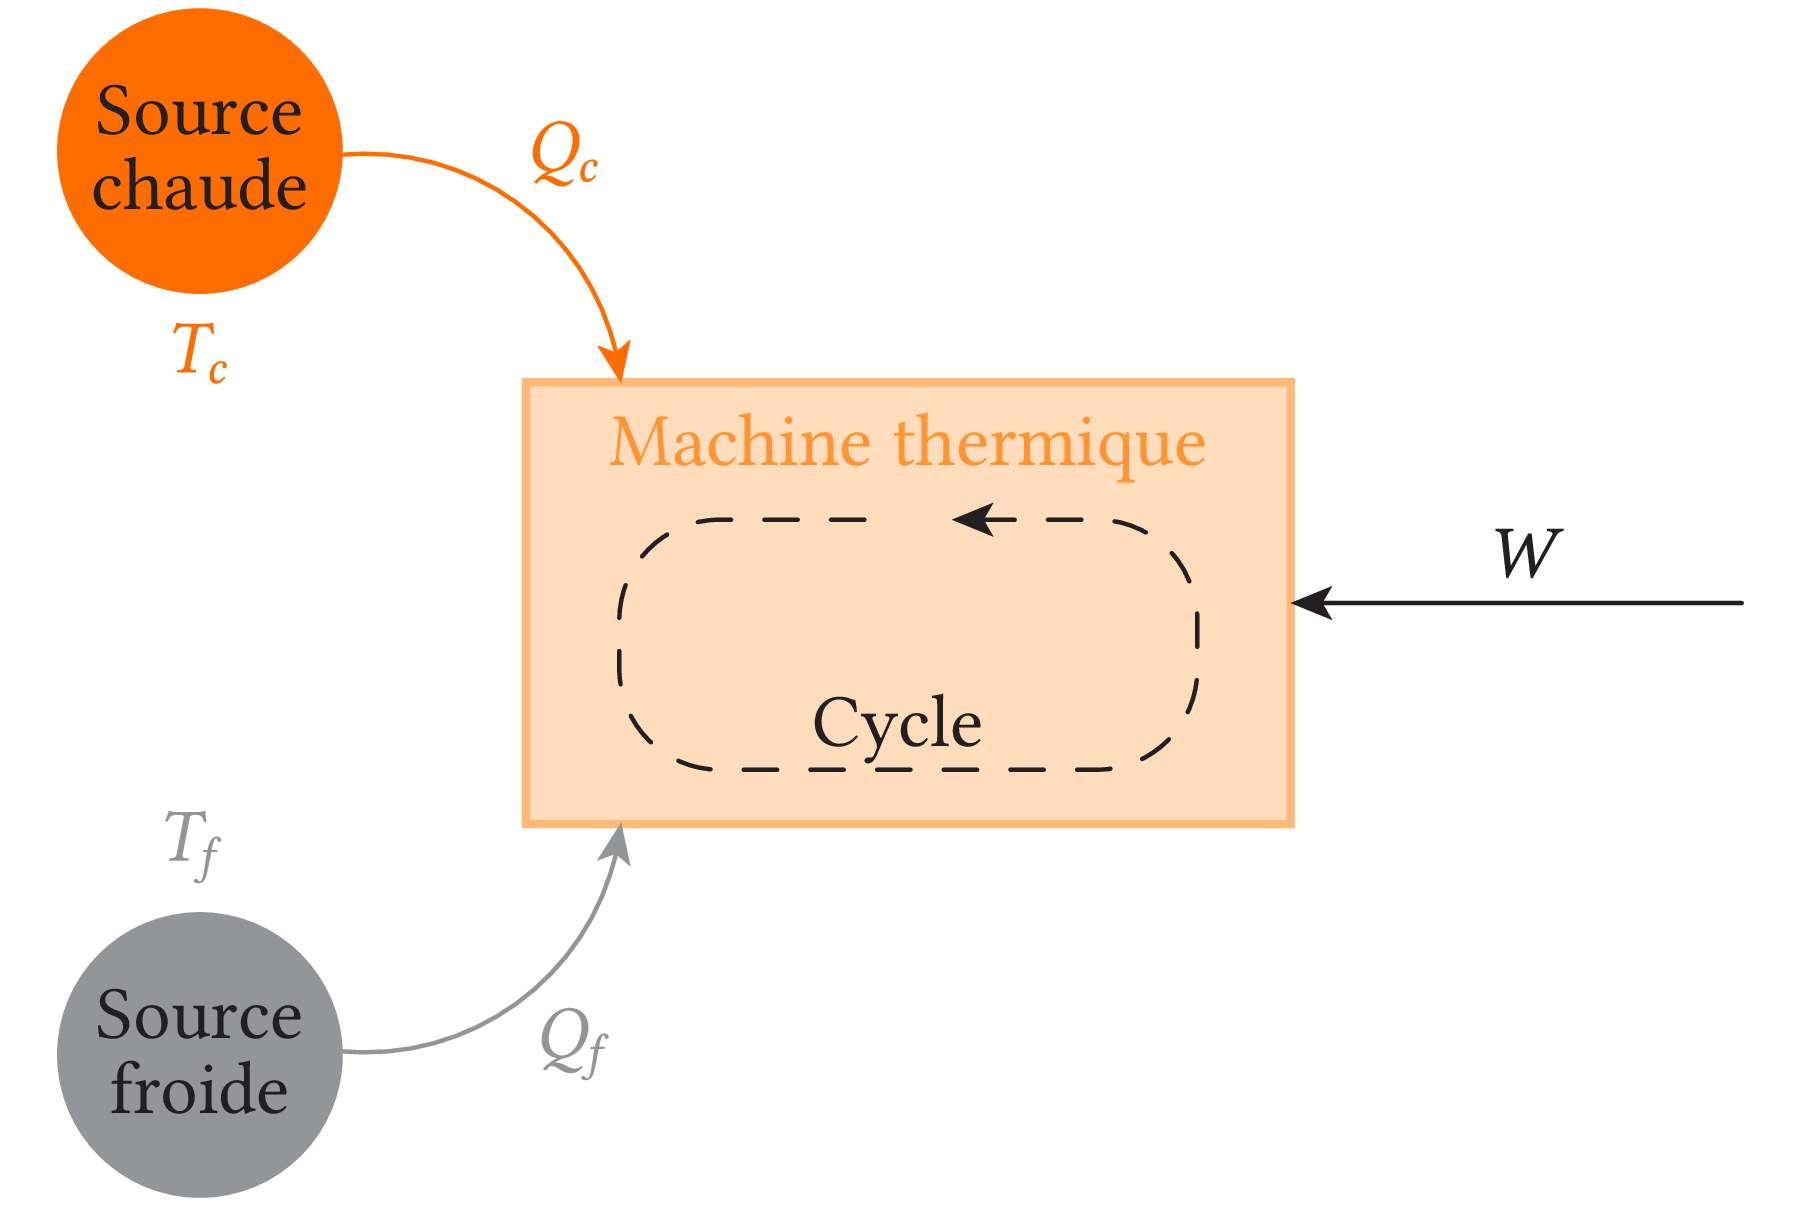
\includegraphics[width=0.65\linewidth]{Figure_Chap19_1.png}
    \caption{Machine thermique ditherme. Source : Fillette, Froustey et Roussille (2023).}
\end{figure}

Les machines thermiques dithermes font intervenir des transferts thermiques avec deux sources : une source chaude à $T = T_c$ et une source froide à $T = T_f$. On note $Q_c$ et $Q_f$ le transfert thermique vers le fluide au contact de ces deux sources.

C'est le cas, par exemple, d'un réfrigérateur : on consomme de l'énergie électrique afin de réaliser un transfert thermique depuis la source froide vers la source chaude.

\begin{definition}
    On définit l'efficacité d'une machine thermique ditherme comme : 
    \begin{equation}
        e = \frac{E_{utile}}{E_{fournie}}
    \end{equation}
    où $E_{utile}$ est l'énergie obtenue à l'aide de la machine, et $E_{fournie}$ est l'énergie fournie à la machine.
\end{definition}

\begin{capex}
En appliquant les principes de la thermodynamique au fluide contenu dans la machine ditherme, déterminer l'efficacité maximale d'un réfrigérateur.
\end{capex}

\begin{solution}
On peut écrire l'efficacité du réfrigérateur comme le rapport entre l'énergie reçue de la source froide, et le travail électrique fourni :
\begin{equation}
    e = \frac{Q_f}{W}
\end{equation}
Nous pouvons par ailleurs établir des relations reliant ces quantités. Le premier principe implique :
\begin{equation}
    \Delta U = 0 = W + Q_f + Q_c
\end{equation}
et
\begin{equation}
    \Delta S = 0 = S_{echangee} + S_{creee}
\end{equation}
Or :
\begin{equation}
    S_{echangee} = \frac{Q_f}{T_f} + \frac{Q_c}{T_c}
\end{equation}
et $S_{creee} \ge 0$, d'où :
\begin{equation}
    \frac{Q_f}{T_f} + \frac{Q_c}{T_c} \le 0
\end{equation}
En remplaçant $Q_c$ à l'aide du premier principe, on trouve que :
\begin{equation}
    e = \frac{Q_c}{W} \le \frac{T_f}{T_c-T_f}
\end{equation}
Il s'agit de l'efficacité de Carnot du réfrigérateur : pour améliorer l'efficacité, il faut se rapporcher le plus possible de la réversibilité et avoir une source chaude et une source froide avec des températures aussi proches que possible.
\end{solution}

Pour un moteur, on peut aussi calculer l'efficacité de Carnot, et on montre que :
\begin{proposition}
Dans le cas d'un moteur thermique fonctionnant en cycle fermé, l'efficacité de Carnot est donnée par :
\begin{equation}
    e = 1 - \frac{T_f}{T_c}
\end{equation}
\end{proposition}
\begin{demonstration}
On a toujours $Q_c+Q_f+W=0$ et $Q_f/T_f + Q_c/T_c \le 0$, mais désormais la source chaude fournit l'énergie à la machine, et l'énergie utile est $-W$. Ainsi :
$e = - W/Q_c$.
On a alors :
\begin{equation}
    \frac{Q_c}{T_c} - \frac{W+Q_c}{T_f} \le 0
\end{equation}
ce qui implique directement que $e \le 1-T_f/T_c$.
\end{demonstration}

Ces résultats sont utiles pour décrire certaines machines ou systèmes naturels. Cependant, un grand nombre de machines thermiques fonctionnent en réalité en circuit ouvert, dans tout ou partie de la machine : un fluide ou de la matière traverse en permanence la machine thermique. C'est le cas par exemple d'un réacteur d'avion ou encore d'un échangeur thermique qui sert à refroidir un fluide. L'objet de ce chapitre est de proposer un cadre conceptuel pour l'étude des systèmes ouverts à partir des principes de la thermodynamique.

\section{Principes infinitésimaux}

\subsection{Premier et second principe}

Nous pouvons, dans un premier temps, nous intéresser aux transformations élémentaires d'un système thermodynamique. Cela sera utile par la suite et va nous permettre de bien distinguer deux formes de nombres infiniments petits en physique.

Considérons un système thermodynamique subissant une transormation quasi-statique. Nous rappelons la définition d'une telle transformation :
\begin{definition}[Transformation quasi-statique (rappel)]
    Une transformation thermodynamique est dite quasi-statique si elle correspond à une succession d'états d'équilibre.
\end{definition}

Dans ce cas, nous pouvons étudier la transformation du système entre deux états infiniments proches. Entre ces deux états, le premier principe va s'écrire :
\begin{equation}
    (\Delta U)' = W' + Q'
\end{equation}
où les primes dénotent des quantités infiniment petites. Cette notation n'est pas habituelle en physique, et on a tendance à utiliser deux notations bien distinctes :
\begin{itemize}
    \item La notation $\dd$ est une différentielle : elle indique la variation infinitésimale d'une fonction d'état thermodynamique $F$ entre l'état initial 1 et l'état final 2 supposés infiniment proches : $\dd F = F_2 - F_1$
    \item La notation $\delta$, au contraire, indique une quantité infinitésimale qui ne peut pas s'écrire comme une différentielle mais qui est calculée lors de la transformation $1 \to 2$ : $\delta X = X_{1 \to 2}$
\end{itemize}
\begin{capex}
Ecrire le premier et le second principe sous leur forme infinitésimale, en prenant soin d'utiliser correctement les notations $\dd$ et $\delta$.
\end{capex}
\begin{solution}
\begin{itemize}
    \item On écrira $(\Delta U)' = \dd U$. Il s'agit d'une différentielle ; la variation infinitésimale de l'énergie interne $U$ entre deux états successifs infiniment proches;
    \item Au contraire $W'$ et $Q'$ ne peuvent pas s'écrire de cette manière car ils ne correspondent pas à la variation d'une quantité d'énergie mais à cette énergie directement. On notera ainsi $\delta W$ le travail élémentaire reçu par le système entre les deux états d'équilibre, et $\delta Q$ le transfert thermique reçu par le système au cours de cette même période. 
\end{itemize}

\begin{theorem}[Premier principe infinitésimal]
    Au cours d'une transformation thermodynamique quasi statique, le premier principe s'écrit :
    \begin{equation}
        \dd U + \dd E_p + \dd E_c = \delta W + \delta Q
    \end{equation}
    où $\dd$ indique la variation infinitésimale d'une énergie, alors que $\delta$ indique une quantité infinitésimale d'énergie.
\end{theorem}

Le second principe s'écrit :
\begin{equation}
    \Delta S = S_{echangee} + S_{creee}
\end{equation}
où $\Delta S$ est la variation d'entropie du système, et $S_{echangee}$ et $S_{creee}$ sont les entropies créée et échangées avec l'extérieur lors de la transformation. Comme $S$ est une fonction d'état, sa variation infinitésimale s'écrit comme une différentielle. Au contraire, lors d'une transformation infinitésimale, les quantités d'entropie créée ou échangée sont infiniment petites mais ne correspondent pas à la variation d'une fonction d'état. 

On en déduit le second principe infinitésimal :
\begin{theorem}
    Au cours d'une transformation thermodynamique quasi statique, le second principe s'écrit :
    \begin{equation}
        \dd S = \delta S _{echangee}+ \delta S_{creee}
    \end{equation}
    où $\dd S$ indique la variation infinitésimale de l'entropie totale du système, alors que $\delta S$ indique une quantité infinitésimale d'entropie.
\end{theorem}

\end{solution}

\subsection{Identité thermodynamique}

On peut appliquer ces deux principes infinitésimaux à une transformation réversible sans variation d'énergie mécanique. Pour ce type de transformation, le travail reçu par le système est fonction de la pression extérieure, qui est égale à la pression à l'intérieur du système car le système est à l'équilibre : $\delta W = - p \dd V$ . Le premier principe s'écrit donc :
\begin{equation}
    \dd U = \delta Q - p \dd V
\end{equation}

Par ailleurs la transformation étant réversible, l'entropie créée est nulle et on peut ainsi écrire :
\begin{equation}
    \dd S  = \delta S_{ech} = \frac{\delta Q}{T}
\end{equation}

En combinant les deux équations, on obtient :
\begin{equation}
    \dd U = T \dd S - p \dd V
\end{equation}
En établissant cette propriété, nous avons considéré une transformation réversible. Mais les variations de $U$, de $S$ et de $V$ ne dépendent pas du chemin suivi (réversible ou non) car ce sont des fonctions d'état qui ne dépendent que des variables d'état du système ($T,V,n$). Donc, elles sont les mêmes que le chemin soit réversible ou non. C'est une propriété fondamentale des fonctions thermodynamiques, on la nomme l'identité thermodynamique :

\begin{theorem}[Identité thermodynamique]
    Lors d'une transformation thermodynamique infinitésimale, l'énergie interne $U$, l'entropie $S$, la pression $p$, le volume $V$ et la température $T$ d'un système thermosynamique sont reliées par la relation suivante :
    \begin{equation}
        \dd U = T \dd S - V \dd p
    \end{equation}
\end{theorem}

En utilisant la définition de l'enthalpie $H = U + pV$ et de l'enthalpie libre $G = H - TS$ on obtient les relations suivantes, qui sont utiles :
\begin{align}
    \dd H &= T \dd S + V \dd p\\
    \dd G &= V \dd p - S \dd T
\end{align}

\begin{remark}
    Nous n'allons pas utiliser l'identité thermodynamique et ses dérivées dans le reste du chapitre. Mais ce sont cependant des relations très utiles dans différents contextes.
\end{remark}

\section{Premier principe pour un système ouvert}

Nous allons maintenant utiliser les principes infinitésimaux pour les appliquer au fonctionnement d'une machine à travers laquelle de la matière passe. Cela peut être, par exemple, de l'air qui passe à travers un réacteur d'avion, ou encore des déchets qui passent à travers un incinérateur. On supposera dans toute la suite le régime stationnaire, c'est-à-dire que les propriétés du système ouvert sont indépendantes du temps. La matière s'écoule à travers le système avec un débit massique :
\begin{equation}
    D_m = \frac{\dd m}{\dd t}
\end{equation}
Comme on est en régime stationnaire, la masse à l'intérieur du système est constante, donc le débit massique entrant et sortant doivent être égaux.

 Nous allons considérer que la matière rentre et sort du système selon le même axe $(Ox)$. Nous nous plaçons en régime permanent, c'est-à-dire que le débit de matière à travers le système ainsi que la puissance thermique et mécanique fournies par le système ne varient pas dans le temps.

Le premier principe s'appliquant uniquement à un système fermé, nous allons devoir construire un système fermé pour pouvoir l'appliquer, puis en déduire des informations sur le système ouvert.

\paragraph{Volume de contrôle}

Nous définissons un volume de contrôle $\mathcal{V}_c$ qui contient le dispositif étudié. Le volume de contrôle est fixe et il est traversé par de la matière : il correspond à un système ouvert que nous notons $\mathcal{S}$. Les propriétés de ce système ne dépendent pas du temps car nous sommes en régime permanent. Comme c'est un système ouvert, nous ne pouvons pas lui appliquer le premier principe. Nous devons construire un système fermé auquel nous pourrons l'appliquer.

\begin{figure}[htbp]
    \centering
    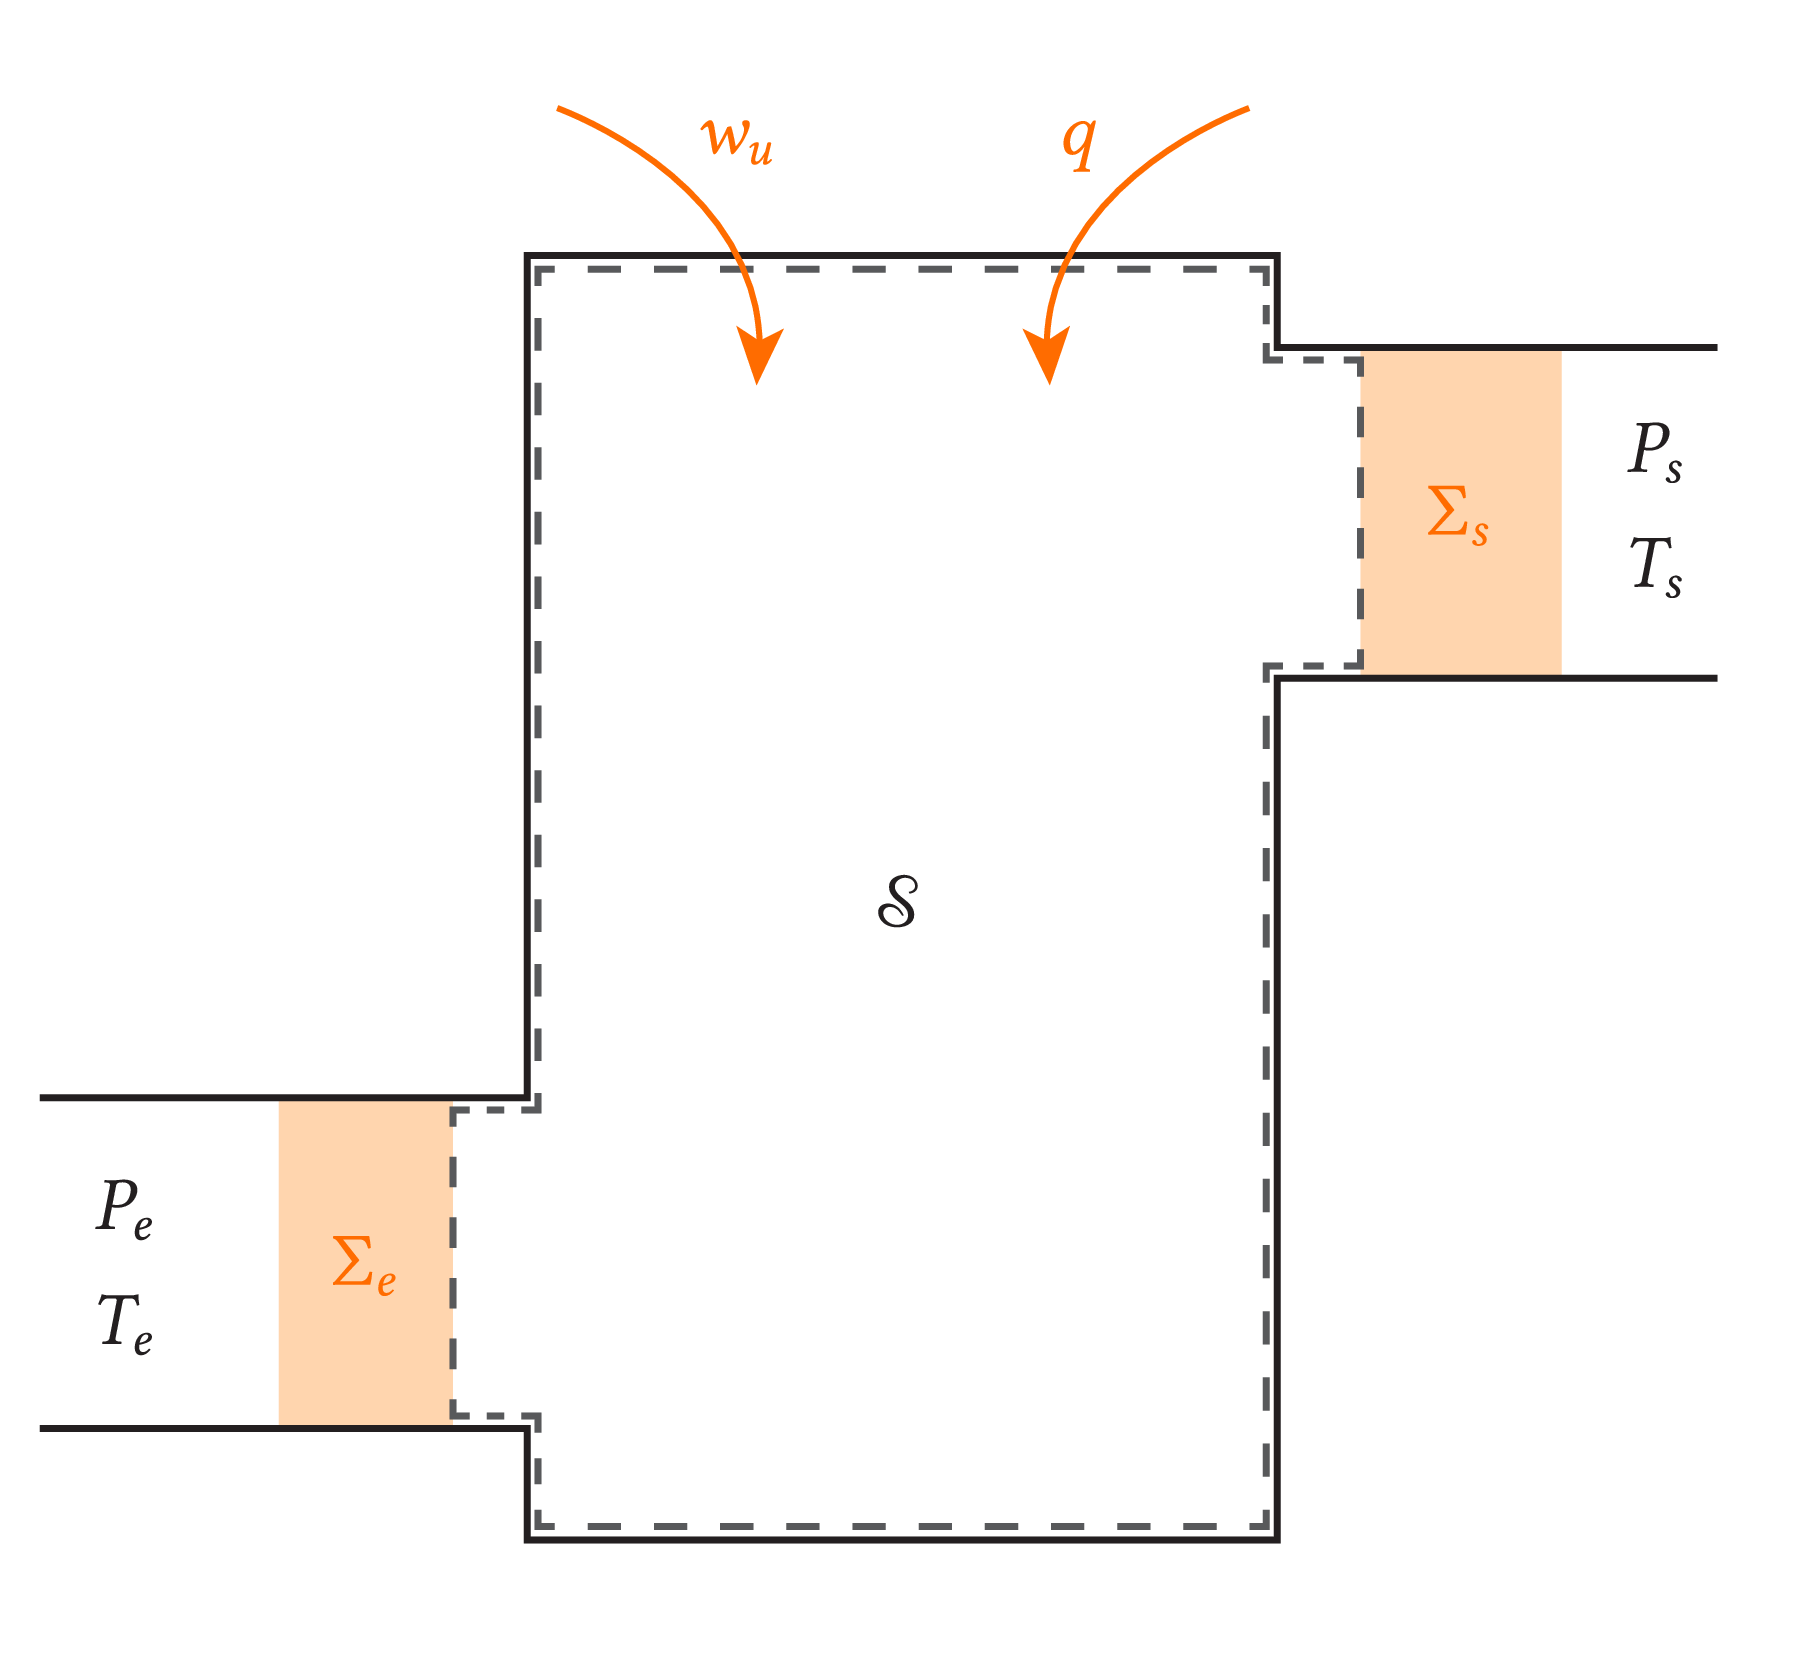
\includegraphics[width=0.6\linewidth]{Figure_Chap18_1.png}
    \caption{Définition du volume de contrôle. Source : Fillette, Froustey et Roussille (2023).}
\end{figure}


\paragraph{Système fermé} Pour cela, nous définissions le système fermé $\Sigma$ qui correspond à l'intérieur du volume de contrôle à l'instant $t$ (le système $\mathcal{S}$) ainsi qu'à la matière qui va rentrer dans le système entre $t$ et $t+\dd t$, que nous notons $\Sigma_e$ : $\Sigma(t) = \mathcal{S} \cup \Sigma_e$. A la différence de $\mathcal{S}$, $\Sigma$ se déplace dans le temps avec la matière qu'il contient. A l'instant $t+\dd t$, le système $\Sigma$ est notamment composé de la matière qui se trouve à l'intérieur du volume de contrôle à $t+\dd t$ ainsi que la matière qui est sortie entre $t$ et $t+\dd t$, que nous notons $\Sigma_s$ : $\Sigma(t+\dd t) = \mathcal{S} + \Sigma_s$.

\begin{capex}
En appliquant le premier principe au système fermé $\Sigma$ en régime stationnaire, relier la variation d'enthalpie massique $h$ du fluide à la puissance thermique $\mathcal{P}_{thermique}$ et mécanique $\mathcal{P}_{mecanique}$ reçue par le fluide dans le système ouvert.
\end{capex}



\begin{solution}
Nous appliquons le premier principe infinitésimal au système fermé $\Sigma$ entre l'instant $t$ et l'instant $t + \dd t$ :
\begin{equation}
    \dd U + \dd E_c + \dd E_p = \delta W + \delta Q
\end{equation}
Or nous pouvons remarquer qu'à l'instant $t$, l'énergie interne du système $\Sigma$ s'écrit :
\begin{align}
    U(\Sigma,t) &= U(\mathcal{S},t) + U(\Sigma_e,t)\\
    &= U(\mathcal{S},t) + \delta m_e \times u_e
\end{align}
où $u_e$ est l'énergie interne massique du fluide entrant dans le système, et $\delta m_e$ est la quantité de masse entrant dans le système entre $t$ et $t+\dd t$. On peut écrire $\delta m_e = D_m \dd t$.
De la même manière :
\begin{align}
    U(\Sigma,t+\dd t) &= U(\mathcal{S},t+\dd t) + U(\Sigma_s,t)\\
    &= U(\mathcal{S},t+\dd t) + \delta m_s \times u_s\\
    &= U(\mathcal{S},t+\dd t) + D_m \dd t \times u_s
\end{align}
Ainsi la variation de l'énergie interne du système fermé $\Sigma$ s'écrit :
\begin{align}
    \dd U &= U(\Sigma,t+\dd t) - U(\Sigma,t) \\
    &= U(\mathcal{S},t+\dd t) - U(\mathcal{S},t) + D_m \dd t \times u_s - D_m \dd t \times u_e \\
    &= D_m \dd t (u_s-u_e)
\end{align}
où nous avons utilisé le fait que nous sommes en régime permanent, si bien que l'énergie interne du système $\mathcal{S}$ est indépendante du temps.

On peut montrer de la même manière que :
\begin{align}
    \dd E_p &=  D_m \dd t (e_{p,s}-e_{p,e}) \\
    \dd E_c &=  D_m \dd t (e_{c,s}-e_{c,e})
\end{align}
où $e_{p,e}$ et $e_{p,s}$ indiquent l'énergie potentielle par unité de masse en entrée et sortie du système, et $e_{c,e}$ et $e_{c,s}$ indiquent l'énergie cinétique par unité de masse en entrée et sortie du système.

L'énergie thermique reçue par le système fermé $\Sigma$ entre $t$ et $t+\dd t$ correspond à l'énergie thermique fournie au volume de contrôle pendant $\dd t$ :
\begin{equation}
    \delta Q = \mathcal{P}_{thermique} \dd t
\end{equation}
où $\mathcal{P}_{thermique}$ est la puissance thermique fournie au volume de contrôle, qui est indépendante du temps (régime permanent).

Le travail reçu par le système pendant $\dd t$ correspond à la somme de deux contributions :
\begin{itemize}
    \item Le travail fourni à l'intérieur du volume de contrôle $\delta W_{machine}$.
    \item Le travail des forces de pression en amont et en aval du système $\delta W_{pres}$
\end{itemize}

De la même manière que pour le transfert thermique, on a :
\begin{equation}
    \delta W_{machine} = \mathcal{P}_{mecanique} \dd t
\end{equation}
où $\mathcal{P}_{mecanique}$ est la puissance mécanique fournie au volume de contrôle.

Le travail des forces de pression s'écrit sous la forme :
\begin{equation}
    \delta W_{pres} = - \int p_{ext} \dd V 
\end{equation}
Comme le volume de contrôle est constant, la variation de volume ne se fait qu'en amont et en aval du système à cause de l'écoulement de matière à travers le volume de contrôle :
\begin{equation}
    \delta W_{pres}= - p_e \dd V_e - p_s \dd V_s
\end{equation}
Si nous notons $\rho_e$ la masse volumique à l'entrée du système, alors $\dd V_e = -\delta m_e/\rho_e = -D_m \dd t/\rho_e$ et de la même manière, $\dd V_s = +D_m \dd t/\rho_s$.
On en déduit :
\begin{equation}
    \delta W_{pres} = D_m \dd t \left(-\frac{p_s}{\rho_s} + \frac{p_e}{\rho_e} \right) = D_m \dd t (-p_s v_s + p_e v_e)
\end{equation}
où nous avons noté $v_e = 1/\rho_e$ le volume massique en entrée du système et $v_s = 1/\rho_s$ le volume massique en sortie du système.

Nous pouvons finalement écrire le premier principe :
\begin{equation}
    D_m \dd t ( u_s - u_e + e_{c,s} - e_{c_e} + e_{m_s} - e_{m,e}) = (\mathcal{P}_{thermique} + \mathcal{P}_{mecanique} ) \dd t + D_m \dd t (-p_s v_s + p_e v_e)
\end{equation}
Nous pouvons simplifier cette expression, en remarquant que les $\dd t$ se simplifient, mais surtout en faisant apparaître l'enthalpie massique $h = u + pv$ :
\begin{equation}
    D_m ( h_s - h_e + e_{c,s} - e_{c_e} + e_{m_s} - e_{m,e}) = \mathcal{P}_{thermique} + \mathcal{P}_{mecanique}
\end{equation}
\end{solution}

Nous avons montré que :
\begin{equation}
        D_m \Delta(h + e_c + e_p) = \mathcal{P}_{thermique} + \mathcal{P}_{mecanique}
\end{equation}
On peut définir le travail utile reçu par unité de masse de fluide, et  le transfert thermique reçu par unité de masse de fluide :
\begin{definition}
    Le travail utile massique reçu par le système ouvert correspond au travail reçu par unité de masse qui traverse le système :
    \begin{equation}
        w_u = \frac{\delta W_u}{\dd m} = \frac{\mathcal{P}_{mecanique}}{D_m}
    \end{equation}
    De même on définit le transfert thermique massique reçu par le système :
    \begin{equation}
        q = \frac{\delta Q}{\dd m} = \frac{\mathcal{P}_{thermique}}{D_m}
    \end{equation}
\end{definition}

Nous aboutissons ainsi à la relation suivante :
\begin{theorem}[Premier principe industriel]
    Soit un système ouvert $\mathcal{S}$ en régime permanent, qui échange de la masse avec l'extérieur via une entrée et une sortie à un débit massique $D_m$. La variation de l'enthalpie massique $h$, de l'énergie cinétique massique $e_c$, et de l'énergie potentielle massique $e_p$ à travers le système est donnée par :
    \begin{equation}
        \Delta(h + e_c + e_p) = w_u + q
    \end{equation}
    où $w_u$ est le travail massique reçu par le système, en considérant uniquement les forces non conservatives autres que les forces de pression.
\end{theorem}

\begin{remark}
    Dans les conditions habituelles des machines indistrielles, on a $|\Delta(e_c + e_p)| \ll \Delta h$. En effet, l'enthalpie massique de vaporisation de l'eau est de l'ordre de $L_v = 2250$\,kJ$\cdot$kg$^{-1}$. Pour avoir une variation d'énergie comparable, il faudrait une vitesse $v = \sqrt{2 L_v} \approx 4$km$\cdot$s$^{-1}$, ou pour l'énergie potentielle, monter l'eau à une altitude $h = L_v/g \approx 250$\,m, ce qui n'est quasiment jamais le cas dans une machine thermique.
\end{remark}

\section{Second principe pour un système ouvert}

On note désormais $s_e$ et $s_s$ l'entropie massique du fluide en entrée et en sortie du système ouvert.

\begin{capex}
Relier la variation d'entropie massique à l'entropie créée et échangée par unité de masse.
\end{capex}

\begin{solution}
De manière analogue à l'énergie interne, l'énergie cinétique et l'énergie potentielle, on peut écrire la variation d'entropie du système comme :
\begin{equation}
    \dd S = D_m (s_s - s_e) \dd t
\end{equation}
Par ailleurs, il n'y a pas d'entropie échangée ou créée au niveau de l'entrée ou de la sortie du système ouvert, on peut donc relier ces deux dernières à l'entropie créée massique dans le système ouvert $s_{creee}$ et l'entropie échangée massique à l'interface entre le système ouvert et l'extérieur par les relations suivantes :
\begin{align}
    \delta S_{echangee} &= s_{echangee} D_m \dd t\\
    \delta S_{creee} &= s_{creee} D_m \dd t
\end{align}

On applique alors le second principe de la thermodynamique au système fermé $\Sigma$ :
\begin{equation}
    \Delta S = \delta S_{echangee} + \delta S_{creee} 
\end{equation}
\end{solution}

On obtient le second principe industriel :
\begin{theorem}[Second principe industriel]
    Soit un système ouvert $\mathcal{S}$ en régime permanent, qui échange de la masse avec l'extérieur via une entrée et une sortie à un débit massique $D_m$. La variation de l'entropie massique $s$ est donnée par :
    \begin{equation}
        \Delta s = s_{echangee} + s_{creee}
    \end{equation}
    où $s_{echangee}$ et $s_{creee}$ sont les entropies échangée avec l'extérieur et créée dans le système par unité de masse de fluide traversant le système.
\end{theorem}

\begin{remark}
    Dans le cas où les échanges thermiques avec l'extérieur se font de façon monotherme, on peut écrire :
    \begin{equation}
        s_{echangee} = \frac{q}{T_{ext}}
    \end{equation}
\end{remark}

En pratique, le second principe va nous permettre de déterminer si une transformation thermodynamique peut se faire spontanément ou non. Il permettra également de calculer l'entropie créée et donc de déterminer si un procédé peut être approximé par une transformation réversible ou non.

\section{Utilisation des diagrammes enthalpiques}

\begin{figure}[htbp]
    \centering
    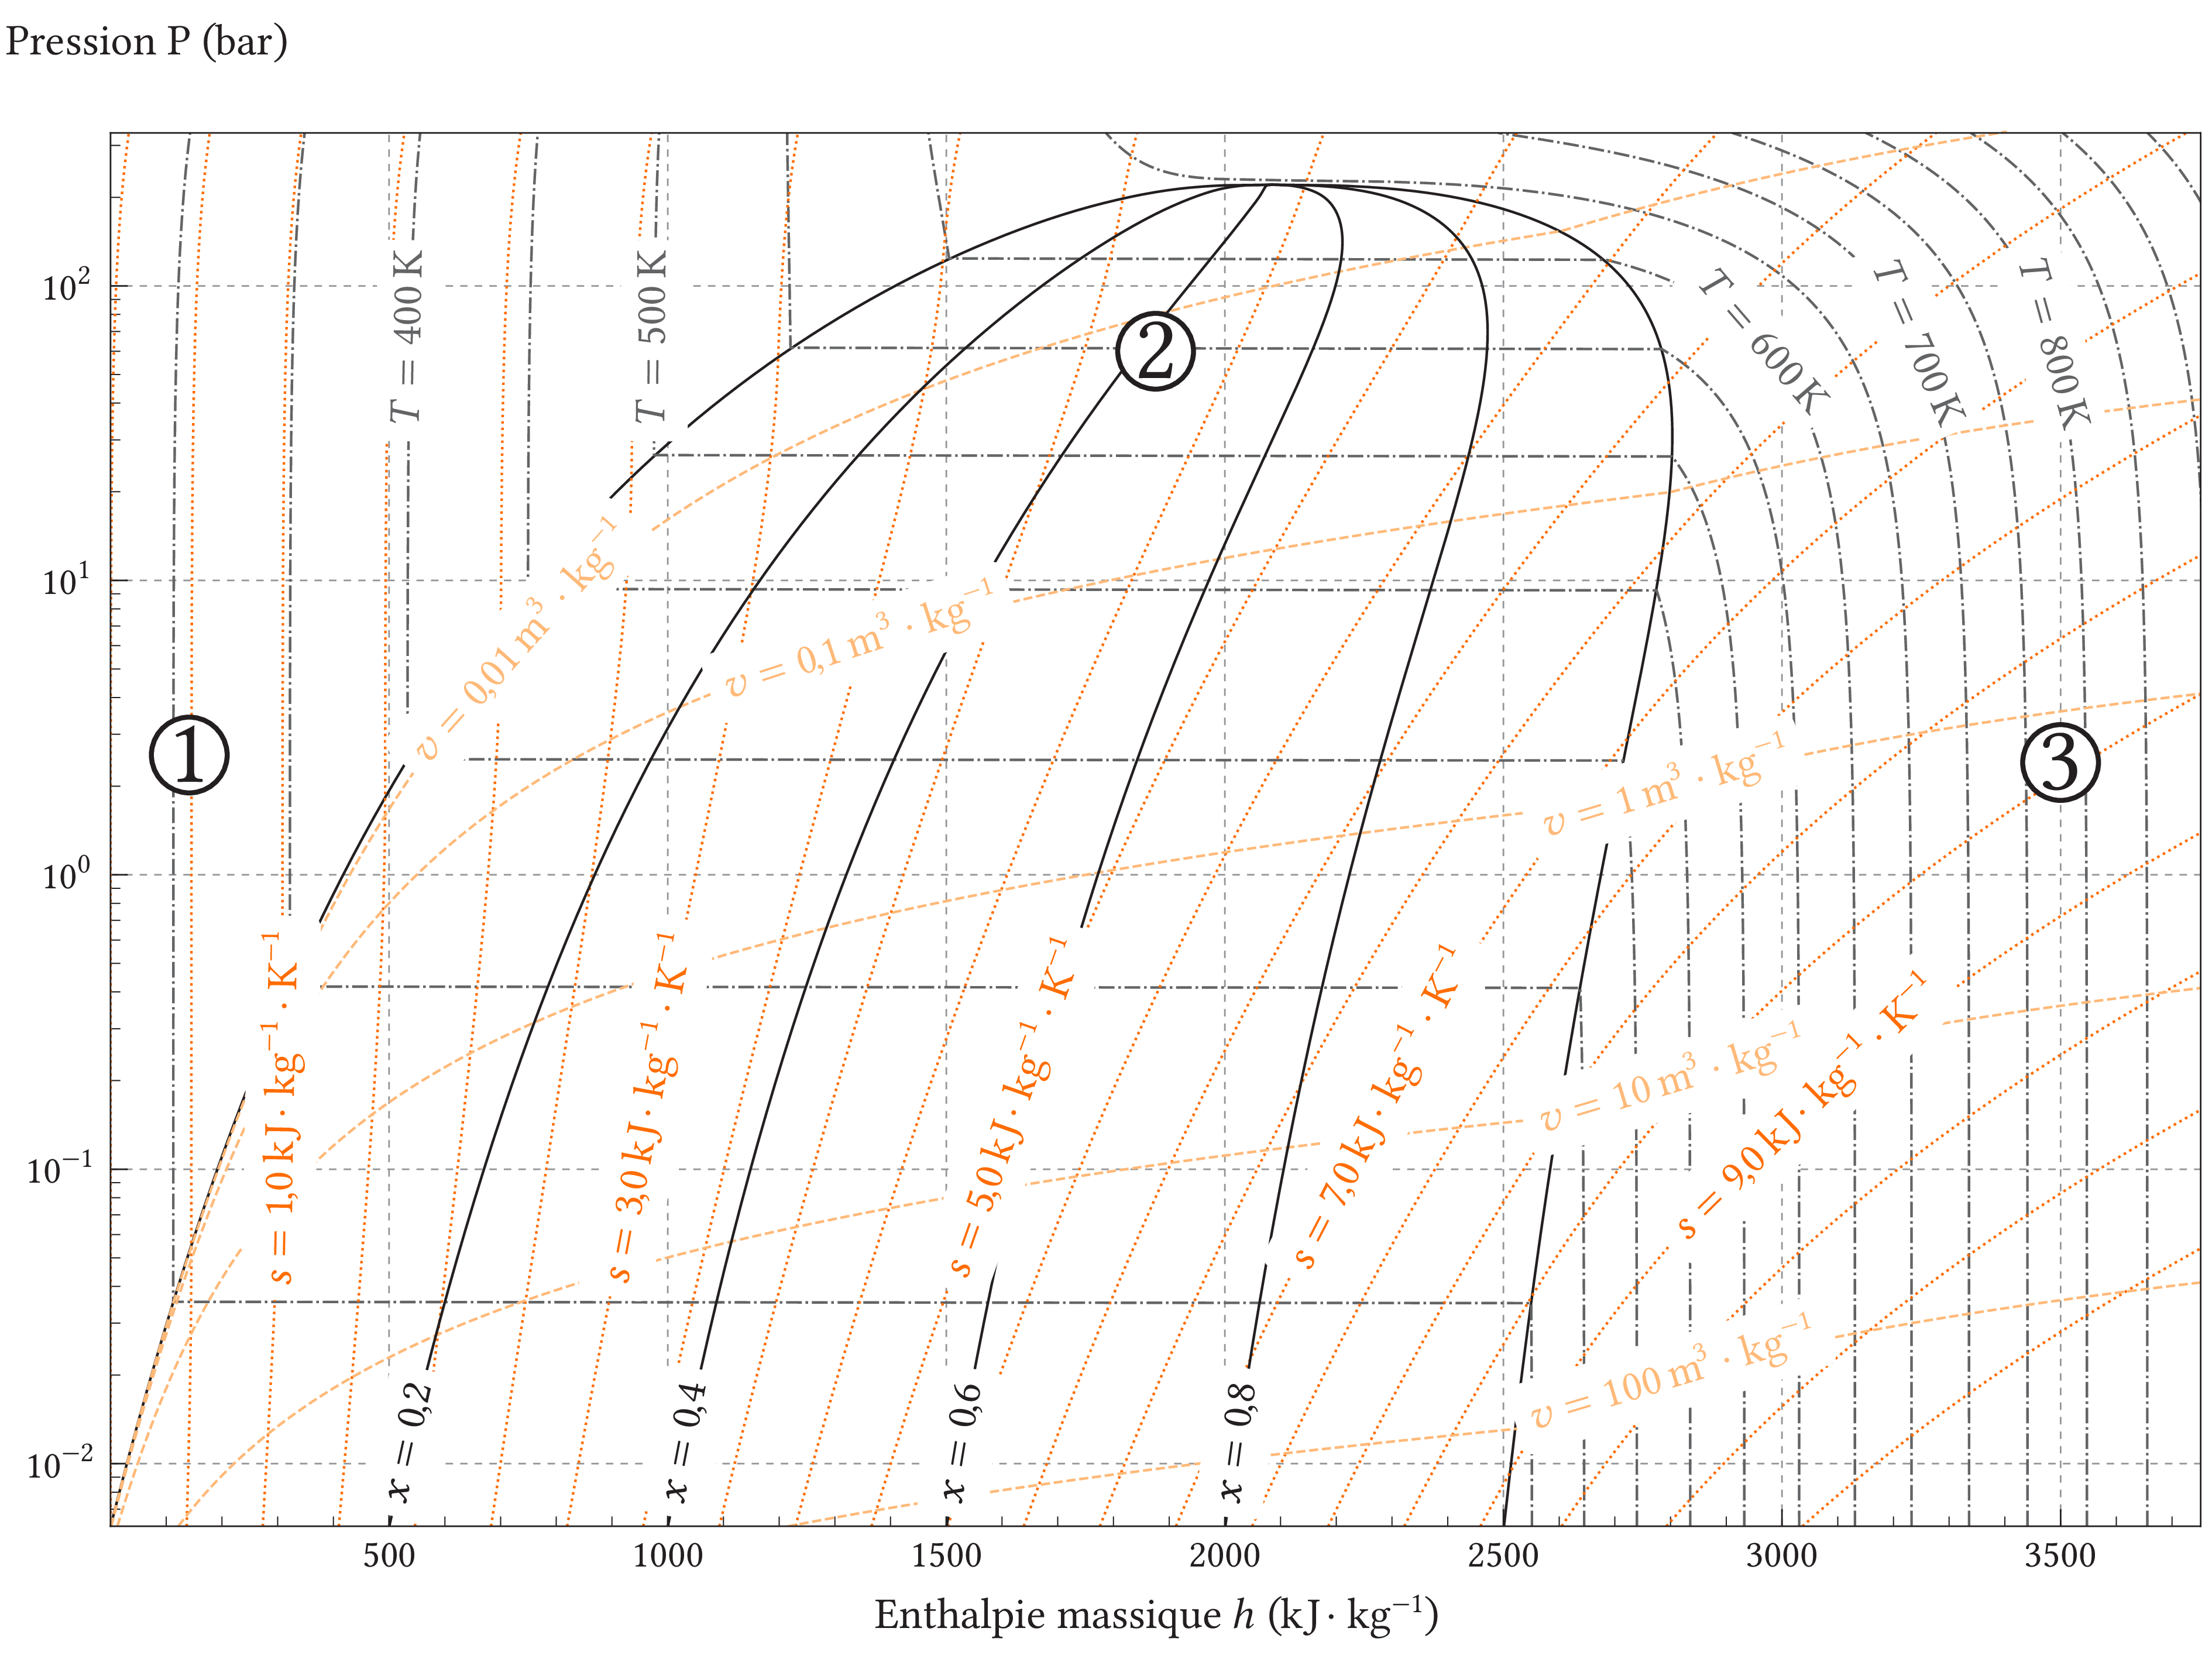
\includegraphics[width=.9\linewidth]{Figure_Chap19_9.png}
    \caption{Diagramme enthalpique de l'eau. Source : Froustey, Fillette, Roussille (2023).}
\end{figure}

L'utilisation de ces principes, et en particulier du premier principe industriel, requiert de connaître l'enthalpie massique d'un fluide en fonction des conditions de pression et de température. Pour cela, on utilise souvent des diagrammes enthalpiques, dans lesquels on fait figurer en fonction de la température et de la pression :
\begin{itemize}
    \item \textbf{Isobares} : ce sont les lignes de pression constante, ici horizontales car la pression est l'axe des ordonnées ;
    \item \textbf{Isothermes} (en gris) : courbes de température constante ;
    \item \textbf{Isochores} (en tirets orange clair) : courbes de volume massique constant ;
    \item \textbf{Isenthalpes} : courbes d'enthalpie massique constante, ici verticales car l'enthalpie massique est l'axe des abcisses ;
    \item \textbf{Isentropes} (en pointillés orange foncé) : courbes d'entropie massique constante.
\end{itemize}
Dans le cas d'un changement d'état, on fait par ailleurs apparaître :
\begin{itemize}
    \item La \textbf{courbe de saturation}, ici en noir, qui délimite les régions liquide (1), gaz (3) et la région biphasée (2).
    \item Les \textbf{isotitres} en noir, correspondant à des lignes où la fraction massique de gaz est constante.
\end{itemize}

\begin{capex}
Démontrer que les isothermes sont verticales dans les zones (1) et (3) en supposant le gaz parfait et les phases condensées idéales, et qu'elles sont horizontales sous la courbe de saturation.
\end{capex}

\begin{solution}
Pour une phase condensée idéale ou pour un gaz parfait, on a :
\begin{equation}
    \dd h = c_p \dd T
\end{equation}
(cette égalité correspond à la deuxième loi de Joule). On en déduite que $h$ est constant si et seulement si $T$ est constante. 

Pour un système diphasé on ne peut pas utiliser la deuxième loi de Joule mais on sait que la pression est égale à la pression de vapeur saturante $p = p_{sat}(T)$, si bien que les courbes de température constante sont confondues avec les courbes de pression constante.

\end{solution}

\begin{remark}
    En pratique on constate que dans certaines régions du diagramme, les isothermes ne sont ni verticales ni horizontales, c'est le cas en particulier dans ou proche de la zone supercritique, où le fluide ne peut être assimilé ni à un gaz parfait ni à une phase condensée idéale.
\end{remark}

De la même manière qu'en première année sur les diagrammes de Clapeyron, on peut utiliser le théorème des moments pour trouver une fraction massique de vapeur sous la courbe de saturation :
\begin{proposition}[Théorème des moments]
On considère un point $M$ de titre vapeur $x$, correspondant à une enthalpie massique $h$. Sur le palier isotherme, on lit $h_{vap}$ et $h_{liq}$. Alors :
\begin{equation}
    x = \frac{h-h_{liq}}{h_{vap}-h_{liq}}
\end{equation}
\end{proposition}

{\begin{wrapfigure}{r}{0.5\textwidth}
    \vspace{-0.5cm}
    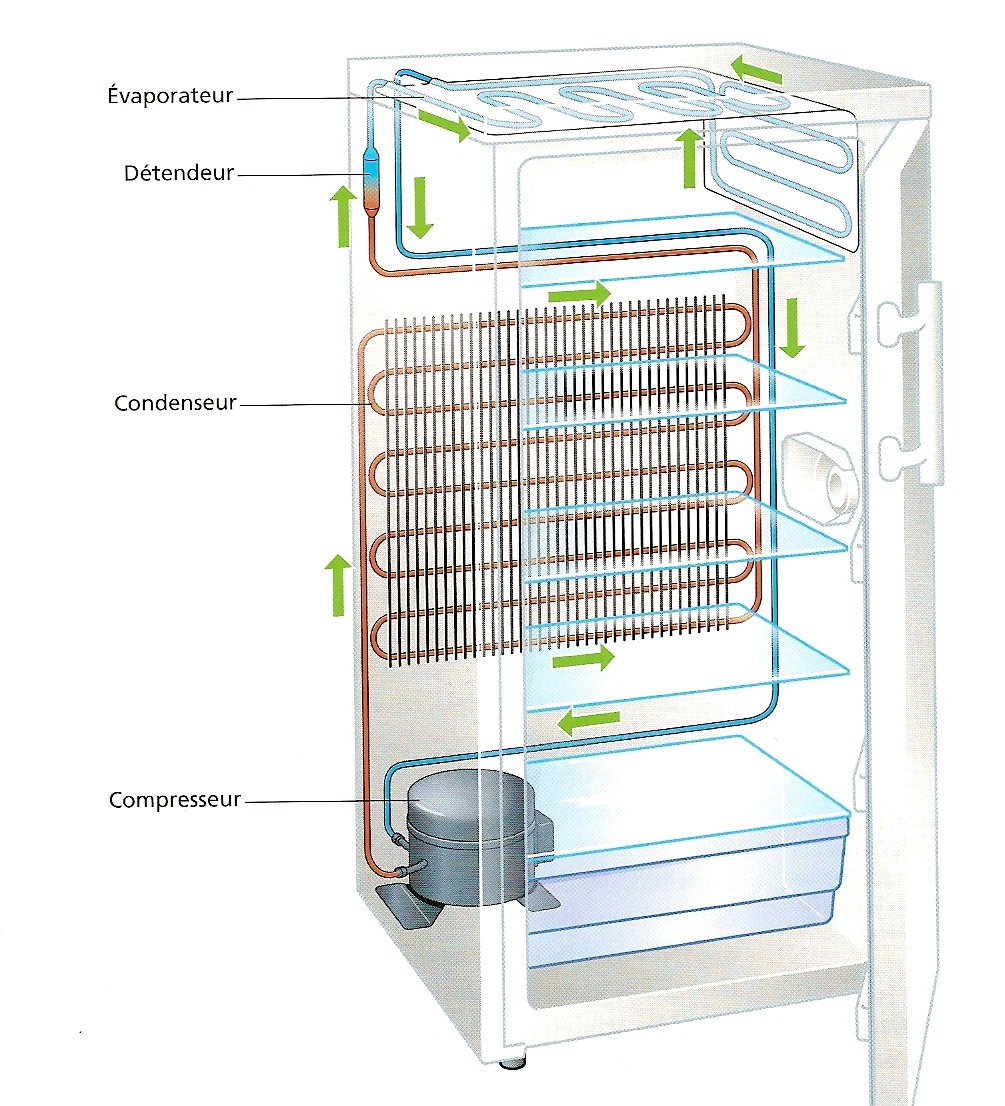
\includegraphics[width=0.99\linewidth]{schema_frigo.jpg}
    \caption{Fonctionnement d'un réfrigérateur. Source : Université du Québec.}
\end{wrapfigure}


\paragraph{Application à une machine frigorifique}

On considère un réfrigérateur contenant le fluide R134a, dont le diagramme est présenté ci-dessous. Le fluide subit un cycle avec les étapes suivantes :
\begin{itemize}
    \item Compresseur : Compression rapide du fluide de 1.3 à 8\,bar
    \item Condenseur : liquéfaction à pression constante au contact de la source chaude. La liquéfaction étant exothermique, de l’énergie est cédée à l’air ambiant.
    \item Détendeur : Le fluide subit une détente adiabatique en l'absence de tout travail extérieur (pas de partie mobile dans le détendeur). La pression redescend à 1.3\,bar. La température diminue à -20$^\circ$C.
    \item Évaporateur : le fluide s'évapore au contact de la source froide, à pression constante. L'évaporation étant endothermique, ceci refroidit l'intérieur du réfrigérateur.
\end{itemize}}

\begin{capex}
A l'aide des différentes étapes du cycle, déterminer l'efficacité du réfrigérateur et la comparer à l'efficacité de Carnot.
\end{capex}

\begin{figure}[p]
    \centering
    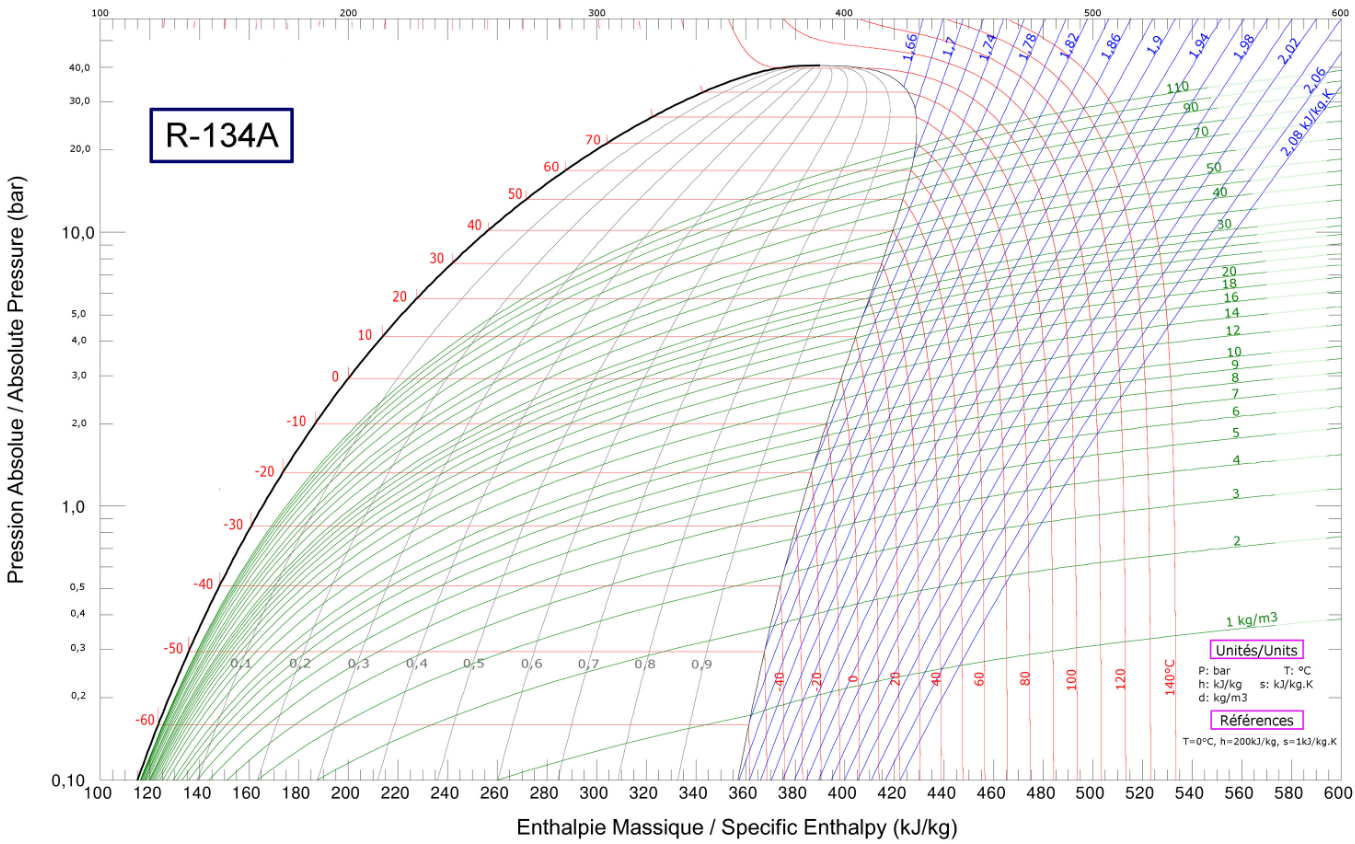
\includegraphics[width=1.5\linewidth,angle=270]{R134a.png}
    \caption{Diagramme enthalpique du R134a. Source : Climalife.}
\end{figure}

\end{document}